\documentclass[12pt]{article}

\newcommand{\undertitle}{Leftovers Group}
\newcommand{\headeright}{Leftovers Group}


\usepackage[utf8]{inputenc} % allow utf-8 input
\usepackage[T1]{fontenc}    % use 8-bit T1 fonts
\usepackage[colorlinks=true, linkcolor=black, citecolor=blue, urlcolor=blue]{hyperref}       % hyperlinks
\usepackage{url}            % simple URL typesetting
\usepackage{booktabs}       % professional-quality tables
\usepackage{amsfonts}       % blackboard math symbols
\usepackage{nicefrac}       % compact symbols for 1/2, etc.
\usepackage{microtype}      % microtypography
\usepackage{lipsum}        % Can be removed after putting your text content
\usepackage{graphicx}
\usepackage{natbib}
\usepackage{doi}
\usepackage{listings}
\usepackage{xcolor}
\usepackage{float}
\setcitestyle{aysep={,}}

\title{Group: Leftovers\\ALU Functions\\Putting It All Together}

\author{Luis Herrera, Philip Ervin\\
CS.3339 Computer Architecture\\
Texas State University\\
}

% Uncomment to remove the date
\date{November 2023}

% Uncomment to override the `A preprint' in the header
\renewcommand{\headeright}{Leftovers Group}
\renewcommand{\undertitle}{Leftovers Group}

\definecolor{codegreen}{rgb}{0,0.6,0}
\definecolor{codegray}{rgb}{0.5,0.5,0.5}
\definecolor{codepurple}{rgb}{0.58,0,0.82}
\definecolor{backcolour}{rgb}{0.95,0.95,0.92}

\lstdefinestyle{mystyle}{
    backgroundcolor=\color{backcolour},   
    commentstyle=\color{codegreen},
    keywordstyle=\color{magenta},
    numberstyle=\tiny\color{codegray},
    stringstyle=\color{codepurple},
    basicstyle=\ttfamily\footsize,
    breakatwhitespace=false,         
    breaklines=true,                 
    captionpos=b,                    
    keepspaces=true,                 
    numbers=left,                    
    numbersep=5pt,                  
    showspaces=false,                
    showstringspaces=false,
    showtabs=false,                  
    tabsize=2
}

\lstset{style=mystyle}

\begin{document}

\maketitle


\newpage
\setcounter{page}{1}

\section{Introduction}
This step of the project combines the efforts described in steps 1 and 2. The goal of this step is to combine previously-created modules onto one virtual circuit and create a control unit to integrate them. For this control unit, operation codes to indicate which operation should be done for each input provided must be defined. With these operation codes and ALU, we have created. This report describes the control unit, operation codes, and overall circuit that comprise our ALU.

\section{Verilog Code For ALU Functions}
\label{sec:headings}

In this section, we will go over every Verilog module which was utilized in the final control circuit.

\subsection{4 Bit AND Gate}

The AND module takes two 4-bit inputs, A and B, and performs a bitwise AND operation between the corresponding bits of these inputs. It also produces a 4-bit output, Y

\lstinputlisting[language=Verilog, basicstyle=\ttfamily\footnotesize]{Verilog/and_4bit.v}


\subsection{4 Bit NAND Gate}

The NAND module takes two 4-bit inputs, A and B, and performs a bitwise NAND operation between the corresponding bits of these inputs. It also produces a 4-bit output, Y.

\lstinputlisting[language=Verilog, basicstyle=\ttfamily\footnotesize]{Verilog/nand_4bit.v}

\subsection{4 Bit OR Gate}

The OR module takes two 4-bit inputs, A and B, and performs a bitwise OR operation between the corresponding bits of these inputs. It also produces a 4-bit output, Y.
\lstinputlisting[language=Verilog, basicstyle=\ttfamily\footnotesize]{Verilog/or_4bit.v}

\subsection{4 Bit NOR Gate}

The NOR module takes two 4-bit inputs, A and B, and performs a bitwise NOR operation between the corresponding bits of these inputs. It also produces a 4-bit output, Y.
\lstinputlisting[language=Verilog, basicstyle=\ttfamily\footnotesize]{Verilog/nor_4bit.v}

\subsection{4 Bit XOR Gate}

The XOR module takes two 4-bit inputs, A and B, and performs a bitwise XOR operation between the corresponding bits of these inputs. It also produces a 4-bit output, Y.
\lstinputlisting[language=Verilog, basicstyle=\ttfamily\footnotesize]{Verilog/xor_4bit.v}

\subsection{4 Bit XNOR Gate}

The XNOR module takes two 4-bit inputs, A and B, and performs a bitwise XNOR operation between the corresponding bits of these inputs.It also produces a 4-bit output, Y.
\lstinputlisting[language=Verilog, basicstyle=\ttfamily\footnotesize]{Verilog/xnor_4bit.v}

\subsection{4 Bit NOT Gate}

The NOT module takes a 4-bit input, A, and produces an inverted  4-bit output, Y. 
\lstinputlisting[language=Verilog, basicstyle=\ttfamily\footnotesize]{Verilog/not_4bit.v}

\subsection{4 Bit Shifter Gate}

The Shifter module takes two 4-bit inputs A and B, where B[3] determines the shift direction, B[2:1] specify the shift amount, and B[0] indicates whether the shift should be filled or emptied. The output Y is the result.

\lstinputlisting[language=Verilog, basicstyle=\ttfamily\footnotesize]{Verilog/newShifter.v}

\subsection{4 Bit Addition Circuit}

The 4-bit addition operation It takes two 4-bit inputs, A and B, along with a carry-in signal Cin, and produces a 4-bit output Sum and a 4-bit output Cout which take the overflow.

\lstinputlisting[language=Verilog, basicstyle=\ttfamily\footnotesize]{Verilog/add_4bit.v}

\subsection{4 Bit Subtraction Circuit}

The 4-bit Subtraction operation accepts two 4-bit inputs, A and B, in addition to a carry-in signal Cin, and generates a 4-bit output Result 4-bit output Cout which take the overflow.

\lstinputlisting[language=Verilog, basicstyle=\ttfamily\footnotesize]{Verilog/sub_4bit.v}

\subsection{4 Bit Multiplication Circuit}

The 4-Bit Multiplication Circuit is designed to take two 4-bit inputs,, and generate a 4-bit product. It does this through a for loop, utilizing the AND operator to calculate partial products for each bit. The final product is then outputted into a 8 bit form named product.

\lstinputlisting[language=Verilog, basicstyle=\ttfamily\footnotesize]{Verilog/multi_4bit.v}

\section{Control Circuit}

\subsection{Control Circuit Verilog Code}
 
The Verilog module, named "integratedModule," is the Control Circuit which performs various 4-bit operations based on the opcode input. It includes modules for AND, NAND, OR, XOR, XNOR, NOR, NOT, SHIFTER, ADD, SUBTRACT, and MULTIPLY. The output Y  return a 4-bit result. To accommodate the 8-bit multiplication results we created a secondary output Y-8bit. The Cin (carry-in) input and Cout (carry out) output is for all modules but only effects the addition, subtraction operations.  \\

The opcode function as such:
\begin{itemize}
    \item[$\bullet$] Input 0000 (Bit 0) is responsible for the AND operation.  
    \item[$\bullet$] Input 0001 (Bit 1) is responsible for the NAND operation. 
    \item[$\bullet$] input 0010 (Bit 2) is responsible for the OR operation. 
    \item[$\bullet$] input 0011 (Bit 3) is responsible for the XOR operation. 
    \item[$\bullet$] input 0100 (Bit 4) is responsible for the XNOR operation. 
    \item[$\bullet$] input 0101 (Bit 5) is responsible for the NOR operation. 
    \item[$\bullet$] input 0110 (Bit 6) is responsible for the NOT operation. 
    \item[$\bullet$] input 0111 (Bit 7) is responsible for the ADD operation. 
    \item[$\bullet$] input 1000 (Bit 8) is responsible for the SUBTRACTION operation. 
    \item[$\bullet$] input 1001 (Bit 9) is responsible for the MULTIPLICATION operation. 
    \item[$\bullet$] input 1010 (Bit 10) is responsible for the SHIFTER operation. 
    
\end{itemize}

\lstinputlisting[language=Verilog, basicstyle=\ttfamily\footnotesize]{Verilog/integratedModule.v}

\subsection{Control Circuit Test Case Verilog Code}

The integrated module Test Case which takes several inputs A, B, Cin, and opcode and produces and 8-bit output Y. The test bench initializes the inputs with specific values, and executes a series of tests in 5 second increments, and monitors the outputs. This test bench tests out all the opcode to verify if they work.

\lstinputlisting[language=Verilog, basicstyle=\ttfamily\footnotesize]{Verilog/benchtest_IntegratedModule.v}

\section{Integrated Module Waveform Tests}

In this section we will showcase the waveforms created using our test benches for each circuit we coded in Verilog. We used GTKWave to create these waveforms.

\begin{figure}[h]
    \centering
    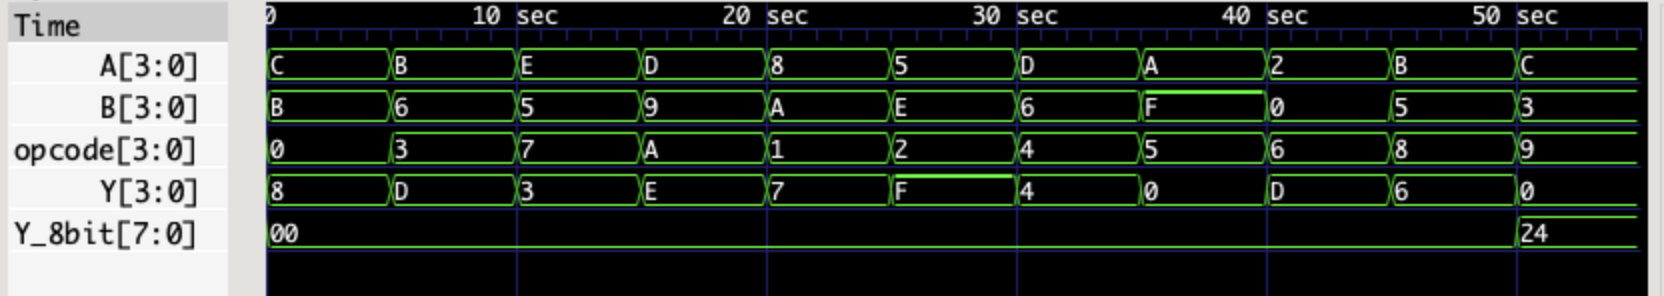
\includegraphics[width = 1.2\textwidth]{../ModuleGTKwave.jpeg}
    \caption{Integrated Module with markers at 5s}
    \label{fig:enter-label}
\end{figure}

Results:
\begin{itemize}
     \item[$\bullet$ ]Test 1: From 0 to 5 seconds, the input A is 1010, input B is 1100 and opcode 0000 which performs the AND Operation outputs Y as 1000. 
     \item[$\bullet$ ]Test 2: From 5 to 10 seconds, the input A is 1011, input B is 0110 and opcode 0011 which performs the XOR Operation outputs Y as 1011.
     \item[$\bullet$ ]Test 3: From 10 to 15 seconds, the input A is 1110, input B is 0101, input Cin is 1, and opcode 1010 which performs the ADDITION Operation outputs Cout is 1 and Y as 0011 .
     \item[$\bullet$ ]Test 4 From 15 to 20 seconds, the input A is 1101, input B is 1001 and opcode 0111 which performs the SHIFT Operation outputs Y as 1110.
     \item[$\bullet$ ]Test 5: From 20 to 25 seconds, the input A is 1000, input B is 1010 and opcode 0001 which performs the NAND Operation outputs Y as 0111.
     \item[$\bullet$ ]Test 6: From 25 to 30 seconds, the input A is 0101, input B is 1110 and opcode 0010 which performs the OR Operation outputs Y as 1111.
     \item[$\bullet$ ]Test 7: From 30 to 35 seconds, the input A is 1101, input B is 0110 and opcode 0100 which performs the XNOR Operation outputs Y as 0100.
     \item[$\bullet$ ]Test 8: From 35 to 40 seconds,  input B is 1111 and opcode 0101 which performs the NOR Operation outputs Y as 1111.
     \item[$\bullet$ ]Test 9: From 40 to 45 seconds, the input A is 0010, input B is 0000 and opcode 0110 which performs the NOT Operation outputs Y as 1101.
     \item[$\bullet$ ]Test 10: From 45 to 50 seconds, the input A is 1011, input B is 0101 and opcode 1000 which performs the SUBTRACTION Operation outputs Y as 0110.
     \item[$\bullet$ ]Test 11: From 50 to 55 seconds, the input A is 1100, input B is 0011 and opcode 1001 which performs the MULTIPLICATION Operation outputs Y-8bit as 100100 .
\end{itemize}

\section{Conclusion}
We are proud to have defined an ALU from first principles in software. For this step, our most significant challenge was defining the formatting of the output and the shift behavior. Defining the operation codes was a methodical process. As a consequence of this project, our team will walk away from this course with improved skills in communication, development, and writing. We also have a new appreciation for the hardware that we are now capable of defining.

\end{document}
